% (c) 2002 Matthew Boedicker <mboedick@mboedick.org> (original author) http://mboedick.org
% (c) 2003-2007 David J. Grant <davidgrant-at-gmail.com> http://www.davidgrant.ca
% (c) 2008 Nathaniel Johnston <nathaniel@nathanieljohnston.com> http://www.nathanieljohnston.com
%
%This work is licensed under the Creative Commons Attribution-Noncommercial-Share Alike 2.5 License. To view a copy of this license, visit http://creativecommons.org/licenses/by-nc-sa/2.5/ or send a letter to Creative Commons, 543 Howard Street, 5th Floor, San Francisco, California, 94105, USA.

\documentclass[letterpaper,11pt]{article}
\newlength{\outerbordwidth}
\pagestyle{empty}
\raggedbottom
\raggedright
\usepackage[svgnames]{xcolor}
\usepackage{framed}
\usepackage{tocloft}
\usepackage{etoolbox}
\usepackage{enumitem}
\usepackage{graphicx}
\usepackage{multirow}
\usepackage{marvosym}
\usepackage{fontawesome5}
\usepackage{hyperref}

\newcommand\fboxpic{\fcolorbox{lightgray}{white}}

\robustify\cftdotfill




%-----------------------------------------------------------
%Edit these values as you see fit

\setlength{\outerbordwidth}{3pt}  % Width of border outside of title bars
\definecolor{shadecolor}{gray}{0.85}  % Outer background color of title bars (0 = black, 1 = white)
\definecolor{shadecolorB}{gray}{0.97}  % Inner background color of title bars


%-----------------------------------------------------------
%Margin setup

\setlength{\evensidemargin}{-0.25in}
\setlength{\headheight}{0in}
\setlength{\headsep}{0in}
\setlength{\oddsidemargin}{-0.25in}
\setlength{\paperheight}{11in}
\setlength{\paperwidth}{8.5in}
\setlength{\tabcolsep}{0in}
\setlength{\textheight}{9.5in}
\setlength{\textwidth}{7in}
\setlength{\topmargin}{-0.3in}
\setlength{\topskip}{0in}
\setlength{\voffset}{0.1in}


%-----------------------------------------------------------
%Custom commands
\newcommand{\resitem}[1]{\item #1 \vspace{-2pt}}
\newcommand{\resheading}[1]{\vspace{8pt}
  \parbox{\textwidth}{\setlength{\FrameSep}{\outerbordwidth}
    \begin{shaded}
\setlength{\fboxsep}{0pt}\framebox[\textwidth][l]{\setlength{\fboxsep}{4pt}\fcolorbox{shadecolorB}{shadecolorB}{\textbf{\sffamily{\mbox{~}\makebox[6.762in][l]{\large #1} \vphantom{p\^{E}}}}}}
    \end{shaded}
  }\vspace{-5pt}
}
\newcommand{\ressubheading}[4]{
\begin{tabular*}{6.5in}{l@{\cftdotfill{\cftsecdotsep}\extracolsep{\fill}}r}
		\textbf{#1} & #2 \\
		\textit{#3} & \textit{#4} \\
\end{tabular*}\vspace{-6pt}}


\usepackage[T1]{fontenc}
\usepackage[utf8]{inputenc}
\usepackage{helvet}

\begin{document}

\begingroup
\renewcommand{\arraystretch}{1.2}
\begin{tabular*}{7in}{l@{\extracolsep{\fill}}rr}
\sffamily{\textbf{\Huge Thomas Holterbach}} & & \multirow{6}{*}{\fboxpic{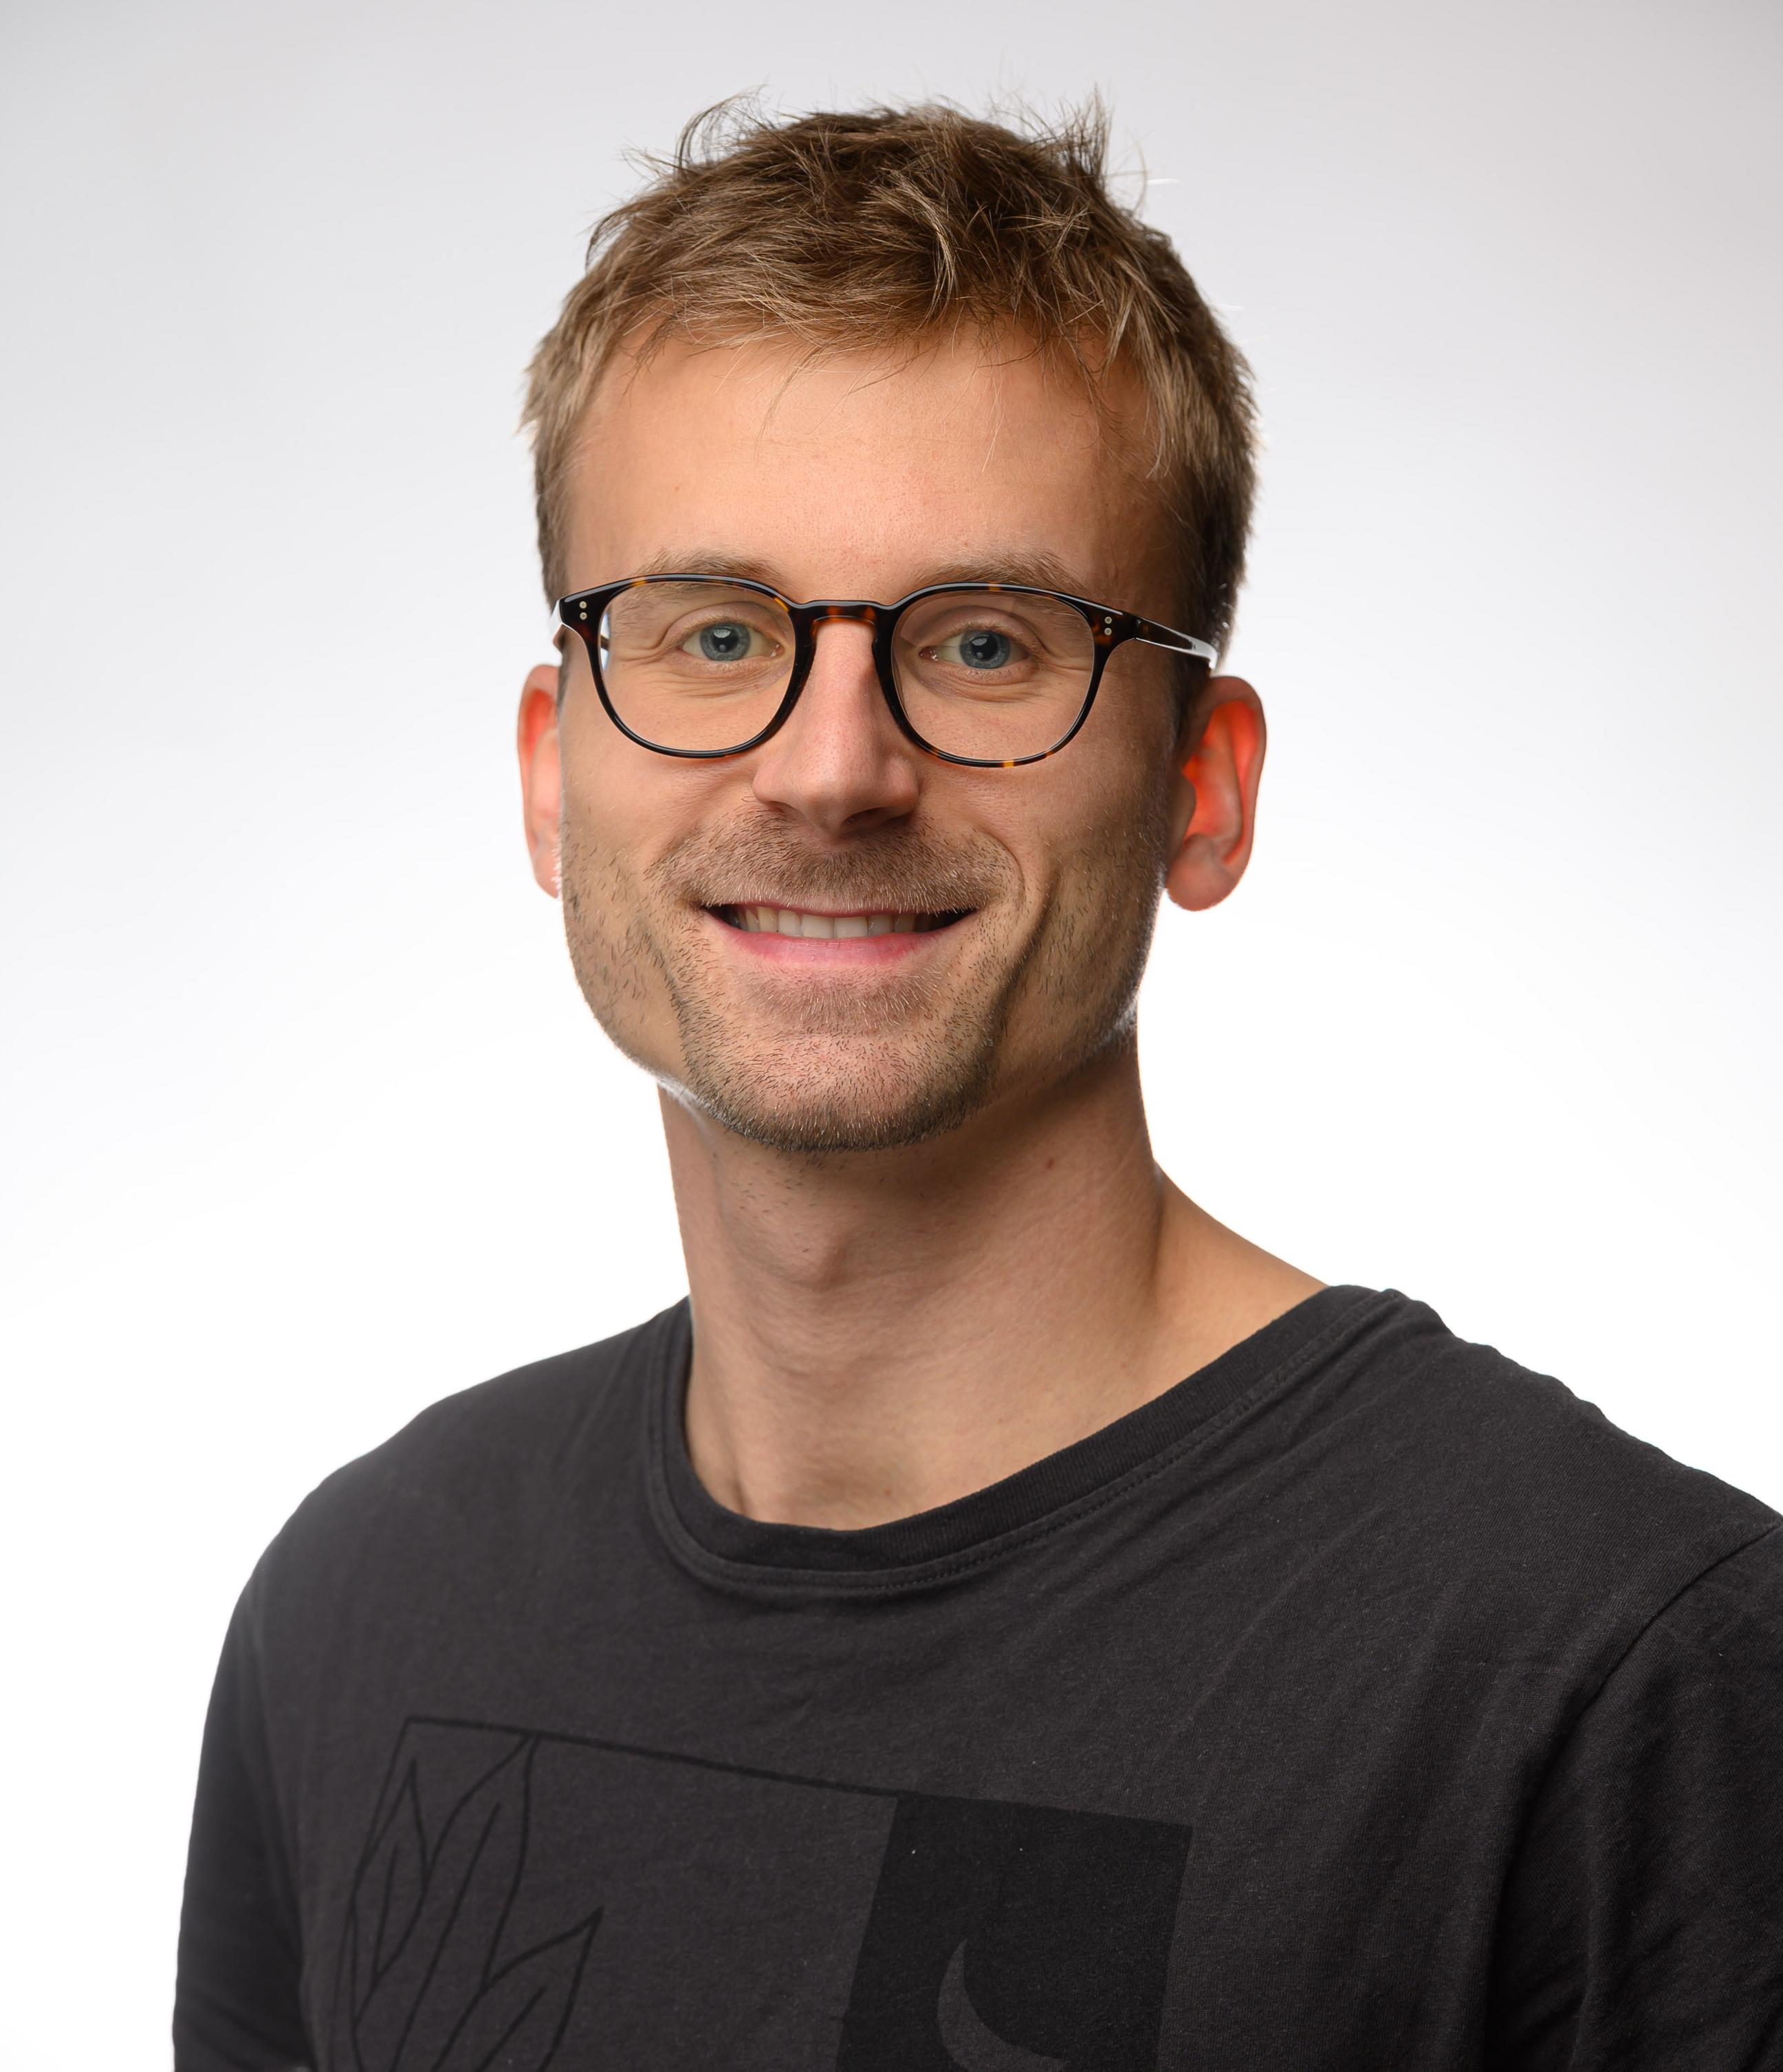
\includegraphics[width=3.5cm]{thomas_picture_zoom2.jpg}}} \\[5pt]
\multicolumn{2}{c}{\sffamily{\large Postdoctoral researcher at the University of Strasbourg ~~~~~~~~~~~~~~~~~~~~~~~~~~~~~~}}  &   \\
&  & \\
&  & \\
&  & \\
& \sffamily{ \sffamily{\Letter~~\small \textcolor{darkgray}{\textit{thomasholterbach@gmail.com}}}} & \\
% & \sffamily{ \sffami	ly{\Large \ComputerMouse \small~~\textcolor{darkgray}{\textit{thomasholterbach.eu}}}} & \\
& \sffamily{ \sffamily{\small \textcolor{darkgray}{\textit{French, born on 31 July 1991}}}} &
% \sffamily{\sffamily{French, 28 years old} & \\

% \renewcommand{\arraystretch}{-1}


%& born on 31 July 1991\\
%& French \\
%&   Last update: \textbf{\today}\\
\end{tabular*}
\endgroup
\\

\vspace{0.2cm}

%%%%%%%%%%%%%%%%%%%%%%%%%%%%%%
\resheading{Research Interests}
\vspace{-0.3cm}

\renewcommand{\arraystretch}{1.2}
\begin{tabular*}{7in}{p{0.3cm}p{10cm}p{8cm}}
    & \\
& \sffamily{$\bullet$~~Internet routing, architecture and security} & \sffamily $\bullet$~~Software-defined networking \\
& \sffamily $\bullet$~~Network traffic measurements and analysis & \sffamily $\bullet$~~Programmable network hardware \\
& \sffamily $\bullet$~~Artificial intelligence for networking & \sffamily $\bullet$~~Algorithm design and optimisation \\
\end{tabular*}

%%%%%%%%%%%%%%%%%%%%%%%%%%%%%%

%%%%%%%%%%%%%%%%%%%%%%%%%%%%%%
\resheading{Education}
%%%%%%%%%%%%%%%%%%%%%%%%%%%%%%
\begin{itemize}[label={},leftmargin=3mm]
\setlength\itemsep{1.5em}


\item

    \begin{tabular*}{6.5in}{l@{\cftdotfill{\cftsecdotsep}\extracolsep{\fill}}r}
    		\sffamily \textbf{Doctoral degree in Computer Science}, ETH Z{\"u}rich, Switzerland & \sffamily Aug. 2021\\
    		% \sffamily \textit{Networked Systems Group} & \\
    		\sffamily Advised by Prof. Laurent Vanbever in the Networked Systems Group & \sffamily \\
    		\sffamily $\bullet$~~Passed the Machine Learning (8 credits) \& Data Mining (4 credits) courses & \\

    \end{tabular*}\vspace{-10pt}

\item

    \begin{tabular*}{6.5in}{l@{\cftdotfill{\cftsecdotsep}\extracolsep{\fill}}r}
    		\sffamily \textbf{Master degree in Computer Science}, University of Strasbourg, France & \sffamily June 2014\\
    		\sffamily{Specialized in Networks and Embedded systems} & \sffamily \\
    		\sffamily With honors. Ranked 2'/15. Grade: 15.2/20 & \\
            & \\
    		% Master Thesis advised by Dr. Pascal Merindol: & \\
    		% Towards Efficient Algorithms for Loop-Free Convergence in Link-State IP Networks & \\

    \end{tabular*}\vspace{-25pt}

\item

    \begin{tabular*}{6.5in}{l@{\cftdotfill{\cftsecdotsep}\extracolsep{\fill}}r}
    		\sffamily \textbf{Bachelor degree in Computer Science}, University of Strasbourg, France & \sffamily June 2012\\
    		\sffamily Ranked 5'/50. Grade: 13.87/20 & \sffamily\\

    \end{tabular*}\vspace{-10pt}

\item

    % \begin{tabular*}{6.5in}{l@{\cftdotfill{\cftsecdotsep}\extracolsep{\fill}}r}
    % 		\sffamily \textbf{Baccalauréat} (French secondary school diploma) & \sffamily July 2009 \\
    % 	    \sffamily With honors. Grade: 14.57/20 & \\
    % \end{tabular*}\vspace{-10pt}

\end{itemize}

%%%%%%%%%%%%%%%%%%%%%%%%%%%%%%
\resheading{Professional Experience}
%%%%%%%%%%%%%%%%%%%%%%%%%%%%%%
\begin{itemize}[label={},leftmargin=3mm]
\setlength\itemsep{1.5em}

\item

    \begin{tabular*}{6.5in}{l@{\cftdotfill{\cftsecdotsep}\extracolsep{\fill}}r}
    		\sffamily \textbf{Postdoctoral researcher}, University of Strasbourg, France & \sffamily Sept. 2021 -\\
    		% \sffamily \textit{Networked Systems Group} & \\
    		\sffamily Advised by Prof. Cristel Pelsser in the Computer Networks Group & \sffamily Jan. 2025\\
			\sffamily $\bullet$~~I developed a system to quickly detect forged-origin hijacks. & \\
			\sffamily The system is open source and runs at \href{https://dfoh.uclouvain.be/}{\textit{dfoh.uclouvain.be/}}. & \\
			\sffamily $\bullet$~~I developed a system to select which BGP vantage points to use when & \\
			\sffamily  measuring Internet routing. The system runs at \href{https://bgproutes.io}{\textit{bgproutes.io}}. & \\

    \end{tabular*}\vspace{-10pt}

\item

    \begin{tabular*}{6.5in}{l@{\cftdotfill{\cftsecdotsep}\extracolsep{\fill}}r}
    		\sffamily \textbf{Postdoctoral researcher and Instructor}, Georgia Tech, GA, USA & \sffamily Sept. 2022 -\\
    		% \sffamily \textit{Networked Systems Group} & \\
    		\sffamily Advised by Prof. Alberto Dainotti in the Internet Intelligence Lab & \sffamily Dec. 2022\\
			\sffamily $\bullet$~~I researched how to build a data-driven network Telescope. & \\
			\sffamily $\bullet$~~I was an instructor in a Master-level class about Internet routing and P4.  & \\

    \end{tabular*}\vspace{-10pt}

\item

\begin{tabular*}{6.5in}{l@{\cftdotfill{\cftsecdotsep}\extracolsep{\fill}}r}
		\sffamily \textbf{Teaching Assistant}, ETH Z{\"u}rich, Switzerland & \sffamily Feb. 2022 -\\
		\sffamily Advised by Prof. Laurent Vanbever in the Networked Systems Group & \sffamily Apr. 2022\\
		\sffamily $\bullet$~~I operated the "mini-Internet" platform in a class with >150 students.  & \\
		\sffamily The platform is open source \href{https://github.com/nsg-ethz/mini_internet_project}{(\textit{mini-inter.net})} and used in many universities world-wide.  & \\

\end{tabular*}\vspace{-6pt}


\item

    \begin{tabular*}{6.5in}{l@{\cftdotfill{\cftsecdotsep}\extracolsep{\fill}}r}
    		\sffamily \textbf{Research and Teaching Assistant}, ETH Z{\"u}rich, Switzerland & \sffamily Feb. 2015 -\\
            \sffamily Supervised by Prof. Laurent Vanbever in the Networked Systems Group & \sffamily Aug. 2021\\
    		\sffamily $\bullet$~~I developed a framework to improve the Internet convergence upon failures.  & \\
	        \sffamily ~~~~Published in [2,3,6], see \href{https://blink.ethz.ch}{\textit{blink.ethz.ch}} and \href{https://swift.ethz.ch}{\textit{swift.ethz.ch}} for further information.  & \\
    		\sffamily $\bullet$~~I developed a "mini-Internet" platform to give students hands on experience routers  & \\
    		\sffamily ~~~~configuration.  We published the platform in [5].& \\

    \end{tabular*}\vspace{-6pt}

\item

    \begin{tabular*}{6.5in}{l@{\cftdotfill{\cftsecdotsep}\extracolsep{\fill}}r}
    		\sffamily \textbf{Visiting Student}, University College London, UK  & \sffamily May 2018 - \\
            \sffamily Supervised by Dr. Stefano Vissicchio in the Department of Computer Science & \sffamily July 2018\\
    		\sffamily $\bullet$~~I developed a P4 program to detect Internet failures in the data plane.  & \\
    		\sffamily ~~~~The program is used in [3], and publicly available at \href{https://github.com/nsg-ethz/Blink}{\textit{github.com/nsg-ethz/Blink}}. & \\
    \end{tabular*}\vspace{-6pt}

\item

    \begin{tabular*}{6.5in}{l@{\cftdotfill{\cftsecdotsep}\extracolsep{\fill}}r}
    		\sffamily \textbf{Junior Researcher}, University of California San Diego, CA, USA & \sffamily June 2016 - \\
            \sffamily Supervised by Dr. Alberto Dainotti in the Center for Applied Internet Data Analysis & \sffamily Dec. 2016\\
    		\sffamily $\bullet$~~I measured the Internet convergence time upon failures using & \\
    		\sffamily ~~~~real BGP data as well as a simulator. Results are used in [2].  & \\

    \end{tabular*}\vspace{-6pt}

\item

    \begin{tabular*}{6.5in}{l@{\cftdotfill{\cftsecdotsep}\extracolsep{\fill}}r}
    		\sffamily \textbf{Research Intern}, Internet Initiative Japan, Tokyo, Japan & \sffamily June 2014 - \\
    		\sffamily Supervised by Prof. Cristel Pelsser and Randy Bush & \sffamily Dec. 2014\\
    		\sffamily $\bullet$~~I studied how accurate are Internet measurement platforms  & \\
    		\sffamily ~~~~such as RIPE Atlas, and we published the work in [1].  & \\
    \end{tabular*}\vspace{-6pt}

\item

    \begin{tabular*}{6.5in}{l@{\cftdotfill{\cftsecdotsep}\extracolsep{\fill}}r}
    		\sffamily \textbf{Research Intern}, University of Strasbourg, France & \sffamily  June 2013 - Aug. 2013 \\
    		\sffamily Supervised by Dr. Pascal Merindol in the ICube laboratory & \sffamily \& Jan. 2014 - July 2014\\
    		\sffamily $\bullet$~~I optimized algorithms designed to prevent forwarding loops. & \\
    		 \multicolumn{2}{l}{\sffamily ~~~~Results are presented in my Master thesis: \small \href{https://dropbox.com/s/fuvamzi5sv1hawq/Mthesis.pdf}{\textit{dropbox.com/s/fuvamzi5sv1hawq/Mthesis.pdf}}.} \\
    \end{tabular*}\vspace{-6pt}

\end{itemize}

% \newpage

%%%%%%%%%%%%%%%%%%%%%%%%%%%%%%
\resheading{Publications}
%%%%%%%%%%%%%%%%%%%%%%%%%%%%%%

\vspace{-0.2cm}


\sffamily

\begin{itemize}[label={},leftmargin=3mm]
\setlength\itemsep{1em}

%\item \large \textbf{Conference papers:} \normalsize

\item

\begin{tabular*}{6.5in}{l@{\cftdotfill{\cftsecdotsep}\extracolsep{\fill}}r}
	\textbf{[9] The Next Generation of BGP Data Collection Platforms} in SIGCOMM 2024  & \\
	\faTrophy~Best Paper Award & \\
	T. Alfroy, \underline{T. Holterbach}, T. Krenc, KC Claffy, and C. Pelsser & \\
\end{tabular*}\vspace{-6pt}

\item

\begin{tabular*}{6.5in}{l@{\cftdotfill{\cftsecdotsep}\extracolsep{\fill}}r}
		\textbf{[9] Measuring Internet Routing from the Most Valuable Points} in arXiv 2024  & \\
		\faVideo~Presented at RIPE 85: \href{https://ripe85.ripe.net/archives/video/934/}{\textit{https://ripe85.ripe.net/archives/video/934/}} & \\
	    T. Alfroy, \underline{T. Holterbach}, T. Krenc, KC Claffy, and C. Pelsser & \\
\end{tabular*}\vspace{-6pt}

\item

\begin{tabular*}{6.5in}{l@{\cftdotfill{\cftsecdotsep}\extracolsep{\fill}}r}
		\textbf{[8] A System to Detect Forge-Origin BGP Hijacks} in NSDI 2024  & \\
		\faVideo~Presented at the Routing Security Summit 2023: \href{https://youtu.be/rdQuy6ckI-s?si=orhLmrXGG9fDvxPW}{\textit{https://youtu.be/rdQuy6ckI-s?si=orhLmrXGG9fDvxPW}} & \\
	    \underline{T. Holterbach}, T. Alfroy, A. Phokeer, A. Dainotti and C. Pelsser & \\
\end{tabular*}\vspace{-6pt}

\item

\begin{tabular*}{6.5in}{l@{\cftdotfill{\cftsecdotsep}\extracolsep{\fill}}r}
		\textbf{[7] Internet Science Moonshot: Expanding BGP Data Horizons}, in HotNets 2023 & \\
	    T. Alfroy, \underline{T. Holterbach}, T. Krenc, KC Claffy, C. Pelsser & \\
\end{tabular*}\vspace{-6pt}

\item

\begin{tabular*}{6.5in}{l@{\cftdotfill{\cftsecdotsep}\extracolsep{\fill}}r}
		\textbf{[6] A Framework To Fast Reroute Traffic Upon Remote Outages}, Doctoral Thesis, 2021 & \\
		Available at \href{https://www.research-collection.ethz.ch/handle/20.500.11850/521609}{\textit{research-collection.ethz.ch/handle/20.500.11850/521609}}  & \\
	    T. Holterbach & \\
\end{tabular*}\vspace{-6pt}

\item

\begin{tabular*}{6.5in}{l@{\cftdotfill{\cftsecdotsep}\extracolsep{\fill}}r}
		\textbf{[5] An Open Platform to Teach How the Internet Practically Works} in CCR 2020  & \\
		\faTrophy~One of the three "Best of CCR" papers presented at SIGCOMM 2020 & \\
		\faVideo~Presented at NANOG 78: \href{https://youtu.be/8SRjTqH5Z8M?si=6z0sbgnm6c32Zgu0}{\textit{https://youtu.be/8SRjTqH5Z8M?si\=6z0sbgnm6c32Zgu0}} & \\
	    \underline{T. Holterbach}, T. B{\"u}hler, T. Rellstab and L. Vanbever & \\
\end{tabular*}\vspace{-6pt}

\item

\begin{tabular*}{6.5in}{l@{\cftdotfill{\cftsecdotsep}\extracolsep{\fill}}r}
		\textbf{[4] (Self) Driving Under the Influence: Intoxicating Adversarial Network Inputs}, in HotNets 2019 & \\
	    R. Meier, \underline{T. Holterbach}, S. Keck, M. Stähli, V. Lenders, A. Singla and L. Vanbever & \\
\end{tabular*}\vspace{-6pt}

\item

\begin{tabular*}{6.5in}{l@{\cftdotfill{\cftsecdotsep}\extracolsep{\fill}}r}
		\textbf{[3] Blink: Fast Connectivity Recovery Entirely in the Data Plane} in NSDI 2019  & \\
	    \underline{T. Holterbach}, E. Costa Molero, M. Apostolaki, S. Vissicchio, A. Dainotti and L. Vanbever & \\
\end{tabular*}\vspace{-6pt}

\item

\begin{tabular*}{6.5in}{l@{\cftdotfill{\cftsecdotsep}\extracolsep{\fill}}r}
		\textbf{[2] SWIFT: Predictive Fast Reroute} in SIGCOMM 2017 & \\
	    \underline{T. Holterbach}, S. Vissicchio, A. Dainotti and L. Vanbever & \\
\end{tabular*}\vspace{-6pt}

\item

\begin{tabular*}{6.5in}{l@{\cftdotfill{\cftsecdotsep}\extracolsep{\fill}}r}
		\textbf{[1] Quantifying Interferences Between Measurements on the RIPE Atlas Platform} in IMC 2015 & \\
	    \underline{T. Holterbach}, C. Pelsser, R. Bush and L. Vanbever & \\
\end{tabular*}\vspace{-6pt}

\vspace{6pt}

\end{itemize}

\vspace{-0.6cm}

%%%%%%%%%%%%%%%%%%%%%%%%%%%%%%
\resheading{Posters and demos}
%%%%%%%%%%%%%%%%%%%%%%%%%%%%%%

\begin{itemize}[label={},leftmargin=3mm]
\setlength\itemsep{1em}

\vspace{-0.2cm}

\item

\begin{tabular*}{6.5in}{l@{\cftdotfill{\cftsecdotsep}\extracolsep{\fill}}r}
		\textbf{MVP: Measuring Internet Routing from the Most Valuable Points} in IMC 2022 & \\
	    T. Alfroy, \underline{T. Holterbach} and C. Pelsser & \\
\end{tabular*}\vspace{-6pt}

\item

\begin{tabular*}{6.5in}{l@{\cftdotfill{\cftsecdotsep}\extracolsep{\fill}}r}
		\textbf{Boosting the BGP convergence in SDXes with SWIFT}, in SIGCOMM 2017 & \\
	    P. Mao, R. Birkner, \underline{T. Holterbach} and L. Vanbever & \\
\end{tabular*}\vspace{-6pt}

\item

\begin{tabular*}{6.5in}{l@{\cftdotfill{\cftsecdotsep}\extracolsep{\fill}}r}
		\textbf{Measurement Vantage Point Selection Using A Similarity Metric} in IRTF \& ISOC ANRW & \\
	    \underline{T. Holterbach}, E. Aben, C. Pelsser, R. Bush, L. Vanbever & \\
\end{tabular*}\vspace{-6pt}

\item

\begin{tabular*}{6.5in}{l@{\cftdotfill{\cftsecdotsep}\extracolsep{\fill}}r}
		\textbf{Supercharge me: Boost Router Convergence with SDN}, in SIGCOMM 2015 & \\
	    M. Alan Chang, \underline{T. Holterbach}, M. Happe, L. Vanbever & \\
\end{tabular*}\vspace{-6pt}
%\item \large \textbf{Workshop papers, posters and demos:} \normalsize


\end{itemize}
\vspace{-0.5cm}

\newpage

%%%%%%%%%%%%%%%%%%%%%%%%%%%%%%
\resheading{Skills}
%%%%%%%%%%%%%%%%%%%%%%%%%%%%%%

\begin{itemize}[label={},leftmargin=3mm]
% \setlength\itemsep{0.3em}
\vspace{-0.3cm}

\item \sffamily \large \textbf{Computer Networks:} \normalsize
\vspace{0.1cm}

\item

\renewcommand{\arraystretch}{1.2}
\begin{tabular}{p{4cm}p{12.5cm}}
  Strong Skills & Network protocols and tools, Internet architecture, Software-defined
  networking, Programmable data planes (P4)  \\[5pt]

  Protocols & STP, IP, BGP, OSPF, MPLS, TCP, DNS, OpenFlow, NetFlow, etc  \\[5pt]

  Tools & Quagga/BIRD, Openvswitch, RIPE Atlas, BGPStream, Tcpdump, Netfilter, OpenVPN, etc  \\[5pt]

  Extra & Cisco IOS, Graph algorithms, Network security, Wireless sensor network

\end{tabular}
\vspace{-0.3cm}

\item \sffamily \large \textbf{Computer Science:} \normalsize
\vspace{0.1cm}

\item

\renewcommand{\arraystretch}{1.2}
\begin{tabular}{p{4cm}p{12.5cm}}
  Strong Skills & Python and C programming, UNIX systems, Algorithm design \\[5pt]

  Languages & C, Python, Java, Bash, R, SQL, etc \\[5pt]

  Tools & Virtualbox/KVM, Docker, Vagrant, Valgrind, Git, etc \\[5pt]

  Extra & Machine learning, Data mining and analytics, Hardware programming, SMT solvers, probability and statistics

\end{tabular}





\vspace{-0.4cm}

\item \large \textbf{Languages:} \normalsize
\vspace{0.1cm}

\item

\begin{tabular}{p{4cm}p{12.5cm}}
  French & Mother tongue \\[5pt]
  English & 5+ years of experience in writing, presenting and teaching \\[5pt]
\end{tabular}

\vspace{-0.5cm}

\end{itemize}

\vspace{-0.2cm}

%%%%%%%%%%%%%%%%%%%%%%%%%%%%%%
\resheading{Teaching and Mentoring}
%%%%%%%%%%%%%%%%%%%%%%%%%%%%%%

\begin{itemize}[label={},leftmargin=3mm]
% \setlength\itemsep{0.3em}

\vspace{-0.3cm}

\item \sffamily \large \textbf{Lecture at Georgia Tech:} \normalsize
\vspace{0.1cm}

\item
\begin{tabular*}{6.5in}{l@{\cftdotfill{\cftsecdotsep}\extracolsep{\fill}}r}
		Computer Networks (CS6250) & 2022 \\
		% ETH Z{\"u}rich, with Prof. Laurent Vanbever &\\
\end{tabular*}\vspace{-6pt}

\vspace{0.3cm}

\item \sffamily \large \textbf{Lectures at ETH Z{\"u}rich:} \normalsize
\vspace{0.1cm}

\item
\begin{tabular*}{6.5in}{l@{\cftdotfill{\cftsecdotsep}\extracolsep{\fill}}r}
		Communication Networks & 2016 - 2022\\
		% ETH Z{\"u}rich, with Prof. Laurent Vanbever &\\
\end{tabular*}\vspace{-6pt}

% \vspace{0.1cm}

\item
\begin{tabular*}{6.5in}{l@{\cftdotfill{\cftsecdotsep}\extracolsep{\fill}}r}
		Advanced Topics in Communication Networks & 2018 - 2020\\
		% ETH Z{\"u}rich, with Prof. Laurent Vanbever &\\
\end{tabular*}\vspace{-6pt}

\item
\begin{tabular*}{6.5in}{l@{\cftdotfill{\cftsecdotsep}\extracolsep{\fill}}r}
		Discrete Event Systems & 2019 - 2020\\
		% ETH Z{\"u}rich, with Prof. Laurent Vanbever &\\
\end{tabular*}\vspace{-6pt}

\vspace{0.3cm}

\item \large \textbf{Students supervision:} \normalsize
\vspace{0.1cm}

\item
\begin{tabular*}{6.5in}{l@{\cftdotfill{\cftsecdotsep}\extracolsep{\fill}}r}
		1 Doctoral thesis supervision (Thomas Alfroy, University of Strasbourg)\\
		% ETH Z{\"u}rich, with Prof. Laurent Vanbever &\\
\end{tabular*}\vspace{-6pt}

\item
\begin{tabular*}{6.5in}{l@{\cftdotfill{\cftsecdotsep}\extracolsep{\fill}}r}
		3 Master thesis supervision (all at ETH Zurich)\\
		% ETH Z{\"u}rich, with Prof. Laurent Vanbever &\\
\end{tabular*}\vspace{-6pt}

\item
\begin{tabular*}{6.5in}{l@{\cftdotfill{\cftsecdotsep}\extracolsep{\fill}}r}
		13 Semester thesis supervision (12 at ETH Zurich, 1 at the University of Strasbourg)\\
		% ETH Z{\"u}rich, with Prof. Laurent Vanbever &\\
\end{tabular*}\vspace{-6pt}




\vspace{-0.5cm}

\end{itemize}



% %%%%%%%%%%%%%%%%%%%%%%%%%%%%%%
% \resheading{Students}
% %%%%%%%%%%%%%%%%%%%%%%%%%%%%%%
%
% \begin{itemize}[label={},leftmargin=3mm]
% \setlength\itemsep{1.5em}
%
% \item
%
% \begin{tabular*}{6.5in}{l@{\cftdotfill{\cftsecdotsep}\extracolsep{\fill}}r}
% 		\textbf{Fabian Schleiss (Master thesis)} & \textit{in progress}\\
% 		Data-plane Driven Fast Network Convergence & \\
% 		\textit{ETH Z{\"u}rich, co-advised with Edgar Costa Molero and Prof. Laurent Vanbever} & \\
% \end{tabular*}\vspace{-6pt}
%
% \item
%
% \begin{tabular*}{6.5in}{l@{\cftdotfill{\cftsecdotsep}\extracolsep{\fill}}r}
% 		\textbf{Simon Miescher (Semester thesis)} & 2017\\
% 		A Fast and Loop-Free Convergence upon Remote BGP Disruptions in Large IP Networks & \\
% 		\textit{ETH Z{\"u}rich, co-advised with Prof. Laurent Vanbever} & \\
% \end{tabular*}\vspace{-6pt}
%
% \item
%
% \begin{tabular*}{6.5in}{l@{\cftdotfill{\cftsecdotsep}\extracolsep{\fill}}r}
% 		\textbf{Edgar Costa Molero (Master thesis)} & 2016\\
% 		Improving Load-Balancing Decisions in Data Center Networks Using SDN & \\
% 		\textit{ETH Z{\"u}rich, co-advised with Prof. Laurent Vanbever} & \\
% \end{tabular*}\vspace{-6pt}
%
% \item
%
% \begin{tabular*}{6.5in}{l@{\cftdotfill{\cftsecdotsep}\extracolsep{\fill}}r}
% 		\textbf{Sol\`{e}ne Buet (Semester thesis)} & 2016\\
% 		On Leveraging Machine Learning techniques to predict
%         the extent of Internet failures & \\
% 		\textit{ETH Z{\"u}rich, co-advised with Prof. Laurent Vanbever} & \\
% \end{tabular*}\vspace{-6pt}
%
% \item
%
% \begin{tabular*}{6.5in}{l@{\cftdotfill{\cftsecdotsep}\extracolsep{\fill}}r}
% 		\textbf{Edgar Costa Molero (Semester thesis)} & 2015\\
% 		Improving Load-Balancing Decisions in IP Networks Using SDN & \\
% 		\textit{ETH Z{\"u}rich, co-advised with Prof. Laurent Vanbever} & \\
% \end{tabular*}\vspace{-6pt}
%
% \item
%
% \begin{tabular*}{6.5in}{l@{\cftdotfill{\cftsecdotsep}\extracolsep{\fill}}r}
% 		\textbf{Roman May (Semester thesis)} & 2015\\
% 		Supercharging IP router memory with SDN & \\
% 		\textit{ETH Z{\"u}rich, co-advised with Prof. Laurent Vanbever} & \\
% \end{tabular*}\vspace{-6pt}
%
% \end{itemize}

% \newpage

% \newpage

% %%%%%%%%%%%%%%%%%%%%%%%%%%%%%%
% \resheading{Activities and Services}
% %%%%%%%%%%%%%%%%%%%%%%%%%%%%%%
% \vspace{-0.3cm}

% \begin{itemize}[label={},leftmargin=3mm]
% \setlength\itemsep{1em}

% \item   

% \begin{tabular*}{6.5in}{l@{\cftdotfill{\cftsecdotsep}\extracolsep{\fill}}r}
% 	\textbf{Reviewed five papers} for ACM CoNEXT & 2022  \\
% \end{tabular*}\vspace{-10pt}

% \item   

% \begin{tabular*}{6.5in}{l@{\cftdotfill{\cftsecdotsep}\extracolsep{\fill}}r}
% 	\textbf{TPC Member for the poster session} for ACM IMC & 2022  \\
% \end{tabular*}\vspace{-10pt}

% \item   

% \begin{tabular*}{6.5in}{l@{\cftdotfill{\cftsecdotsep}\extracolsep{\fill}}r}
% 	\textbf{TPC Member for the Artifact Evaluation} for ACM CoNEXT & 2020  \\
% \end{tabular*}\vspace{-10pt}

% \item

% \begin{tabular*}{6.5in}{l@{\cftdotfill{\cftsecdotsep}\extracolsep{\fill}}r}
% 		\textbf{Shadow TPC member} for ACM IMC & 2019  \\
% \end{tabular*}\vspace{-10pt}

% \item

% \begin{tabular*}{6.5in}{l@{\cftdotfill{\cftsecdotsep}\extracolsep{\fill}}r}
% 		\textbf{Occasional Reviewer} for IEEE/ACM ToN and ACM CCR & 2016 - 2020 \\
% \end{tabular*}\vspace{-10pt}

% \item

% \begin{tabular*}{6.5in}{l@{\cftdotfill{\cftsecdotsep}\extracolsep{\fill}}r}
% 		\textbf{CAIDA BGP Hackathon}, San Diego, CA, USA (travel granted) & Feb. 2016\\
% \end{tabular*}\vspace{-10pt}

% \item

% \begin{tabular*}{6.5in}{l@{\cftdotfill{\cftsecdotsep}\extracolsep{\fill}}r}
% 		\textbf{PhD School on Software-defined Networks}, Heracklion, Greece & July 2015\\
% \end{tabular*}\vspace{-10pt}

% \item

% \begin{tabular*}{6.5in}{l@{\cftdotfill{\cftsecdotsep}\extracolsep{\fill}}r}
% 		\textbf{PhD School on Traffic Monitoring and Analysis}, Barcelona, Spain (travel granted) & April 2015\\
% \end{tabular*}\vspace{-10pt}

% \item

% \begin{tabular*}{6.5in}{l@{\cftdotfill{\cftsecdotsep}\extracolsep{\fill}}r}
% 		\textbf{RIPE Atlas Hackathon}, Amsterdam, Netherlands, (travel granted) & March 2015\\
% \end{tabular*}\vspace{-10pt}

% \end{itemize}


% %%%%%%%%%%%%%%%%%%%%%%%%%%%%%%
% \resheading{References}
% %%%%%%%%%%%%%%%%%%%%%%%%%%%%%%

% \begin{itemize}[label={},leftmargin=3mm]
% \setlength\itemsep{1em}

% \item

% References available upon request.
% \end{itemize}


\end{document}
